\chapter {DASAR TEORI}

Pada bab ini, akan dijelaskan dasar teori yang digunakan sebagai landasaan pengerjaan Tugas Akhir ini.

\section{Deskripsi Permasalahan}
Permasalahan yang dibahas pada Tugas Akhir ini adalah perhitungan untuk mencari perimeter polygon terkecil dari sekumpulan titik yang dibatasi di dalam polygon sederhana.
\begin{figure}
	\Centering
	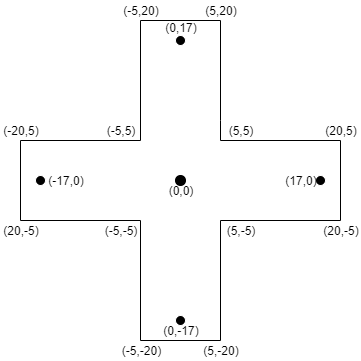
\includegraphics [width=0.5\columnwidth]{bab2/img/contoh-kasus-tanpa-solusi}
	\caption {Ilustrasi contoh kasus tanpa solusi}
	\label {fig:ilustrasi-contoh-kasus-tanpa-solusi}
\end{figure}
\begin{figure}
	\Centering
	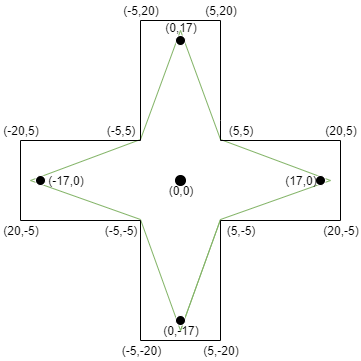
\includegraphics [width=0.5\columnwidth]{bab2/img/contoh-kasus}
	\caption {Ilustrasi contoh kasus}
	\label {fig:ilustrasi-contoh-kasus}
\end{figure}


\begin{algorithm}
	\caption{Faktorial Modulo Prima Naif}
	\label{psdo:factorial_naif}
	\begin{algorithmic}[1]
		\Require $n,\ p$
		\Ensure $n! \textbf{ mod } p$
		\State $f \leftarrow 1$
		\For{ $i \leftarrow 1 \text{ to } N $} 
			\State $ f \leftarrow ( f * i ) \textbf{ mod } p$
		\EndFor \\
		\Return $ f \textbf{ mod } p $
	\end{algorithmic}
\end{algorithm}

Dikarenakan nilai batasan $ N $ pada deskripsi soal cukup besar yaitu $ 10^{11} $, sehingga algoritma naif akan memberikan verdict \textit{Time Limit Excedeed} karena melampaui batas waktu yang telah ditentukan.

\section{Strategi Penyelesaian dengan Multipoint Evaluation}
\label{sec:penyelesaian_multipoint_evaluation}
Pada subbab ini akan dipaparkan mengenai strategi penyelesaian masalah klasik pada daring SPOJ dengan kode FACTMODP dengan \textit{Multipoint Evaluation}. Secara singkat, strategi penyelesaian masalah dari FACTMODP menggunakan \textit{Multipoint Evaluation} terbagi menjadi 4 bagian besar yaitu :
\begin{enumerate}
	\item Perumusan Transformasi Faktorial
	\item Membangun Pohon Polinomial
	\item Evaluasi Pohon Polinomial
	\item Komputasi Faktorial berdasarkan Hasil Evaluasi
\end{enumerate}

Sebagai contoh, pada subbab ini akan menggunakan $ N = 10 $ serta $ P = 10^9 + 7 $ sebagai modulo. Nilai $ N $ dan $ P $ yang dipilih berada didalam batasan yang didefinisikan dalam subbab \ref{sec:batasan_masalah}. Persoalan utama dalam Tugas Akhir ini adalah memodelkan faktorial sedemikian hingga dapat dikomputasi dengan kompleksitas dibawah $ \mathcal{O}{(N)} $.

\subsection{Perumusan Transformasi Faktorial}
\label{sec:perumusan_transformasi_faktorial}
Dimisalkan bilangan bulat positif $ v = \lfloor \sqrt{N} \rfloor $ serta polinomial $ g(x) = \prod_{i=0}^{v-1} (x + vi + 1) $, sehingga didefinisikan persamaan faktorial baru pada persamaan \eqref{eq:persamaan_faktorial_baru}.
\begin{equation}
	N ! = \left( \prod_{i=0}^{v-1} g(i) \right) \cdot \prod_{i=v^2+1}^n i
	\label{eq:persamaan_faktorial_baru}
\end{equation}
Untuk $ N = 10 $, maka nilai polinomial $g(x)$ adalah $$ (x+1)(x+4)(x+7) = (x^3 + 12x^2 + 39x + 28). $$ Berdasarkan persamaan \eqref{eq:persamaan_faktorial_baru}, nilai dari $ 10! = g(0) \cdot g(1) \cdot g(2) \cdot 10 = 3628800 $. 
Menurut \cite{multipoint_evaluation}, nilai dari $ g(0), g(1), \cdots , g(v-1) $ dapat dievaluasi sekaligus, sehingga komputasi $ N! \text{ mod } P $ dapat dipercepat.
\newpage
Dalam algoritma \textit{Multipoint Evaluation}, dibutuhkan pembangunan pohon biner perkalian polinomial, yang selanjutnya disebut pohon polinomial, terlebih dahulu. Pohon polinomial ini dibangun dari titik evaluasi, bukan berdasarkan polinomial yang dievaluasi. Secara umum membangun pohon polinomial menggunakan paradigma \textit{bottom-up}, ilustrasi pembangunan pohon polinomial dapat dilihat pada gambar \ref{fig:ilustrasi-pohon-polinomial}.

\begin{figure}
	\Centering
	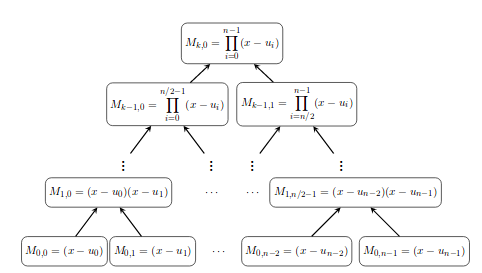
\includegraphics [scale=0.6]{bab2/img/ilustrasi-pohon-polinomial}
	\caption {Ilustrasi Pohon Polinomial}
	\label {fig:ilustrasi-pohon-polinomial}
\end{figure}

\subsection{Membangun Pohon Polinomial}
\label{sec:membangun_pohon_polinomial}
Dimisalkan $ u_0, u_1, \cdots , u_{n-1} $ adalah titik yang akan dievaluasi pada polinomial $ g(x) $. Dalam membangun pohon polinomial, diperlukan polinomial $( x - u_i) $ untuk $ 0 \leq i < n $ sebagai \textit{leaf} dan \textit{node} yang merepresentasikan hasil perkalian dari semua \textit{node} atau \textit{leaf} dibawahnya. 

Polinomial $ M_{i,j} $ menyatakan polinomial dengan tinggi $ i $ dan indeks ke-$ j $ dari kiri pohon. Akar dari pohon merepresentasikan polinomial $ M_{k,0} = \prod_{i=0}^{n-1} (x - u_i) $ dan setiap \textit{leaf} merepresentasikan polinomial $ M_{0,j} = x - u_j $.

Apabila perkalian polinomial berbasis \textit{Fast Fourier Transform},digunakan dalam pseudocode \ref{psdo:general_subproduct_tree}, akan didapatkan algoritma yang efisien. Penjelasan mengenai perkalian polinomial berbasis \textit{Fast Fourier Transform} akan dibahas pada subbab berikutnya.
% TODO : subbab berapa

\begin{algorithm}
	\caption{Membangun Pohon Polinomial (General)}
	\label{psdo:general_subproduct_tree}
	\begin{algorithmic}[1]
		\Require $ N = 2^k, k \in \mathbb{N},\ u_0, u_1, \cdots , u_{n-1} \in R $
		\Ensure $ \text{Pohon Polinomial } M_{i,j} \text{ untuk } 0 \leq i \leq k \text{ dan } 0 \leq j < 2^{k-i} $
		\For {$ j = 0, \cdots , n-1 $} 
			\State $ M_{0,j} \gets (x - u_i) $
		\EndFor
		\For {$ i = 1, \cdots , k $ }
			\For {$ j = 0, \cdots, 2^{k-i}-1 $} 
				\State $ M_{i,j} \gets M_{i-1,2j} \cdot M_{i-1,2j+1}$
			\EndFor
		\EndFor
	\end{algorithmic}
\end{algorithm}

% TODO : subbab berapa.
Pseudocode \ref{psdo:general_subproduct_tree} berlaku apabila $ N $ merupakan bilangan pangkat dua, apabila $ N $ bukan bilangan pangkat dua, maka dapat diterapkan metode rekursi dalam membangun pohon polinomial tersebut, yang dibahas pada subbab berikutnya. Untuk $ N = 10 $, maka pohon polinomial yang dibangun akan terlihat seperti pada gambar \ref{fig:pohon-polinomial-n-10}.  

Secara umum pada step ke-$ m $ dalam membangun pohon polinomial dengan tinggi $ k $, algoritma ini mengalikan $ 2^{k-m} $ pasang polinomial dengan derajat $ 2^{m-1} $. Apabila $ M(n) \simeq \mathcal{O}{(n \text{ log } n)} $ merepresentasikan kompleksitas perkalian polinomial berbasis \textit{Fast Fourier Transform} dengan derajat kurang dari $ n $ dan $ 0 \leq m < k $ maka kompleksitas yang dibutuhkan untuk membangun pohon polinomial ditunjukan pada persamaan \eqref{eq:kompleksitas_pohon_polinomial}.
\begin{equation}
	\begin{aligned}
		& \frac{n}{2}M(2) + \frac{n}{4}M(4) + \cdots + 4M(\frac{n}{4}) + 2M(\frac{n}{2}) \\
		\leq & M(n) + M(n) + \cdots M(n) + M(n) \\
		= & (log_2(n) - 1)M(n) \in \mathcal{O}{(n \text{ log }^2\ n)} \\
	\end{aligned}
	\label{eq:kompleksitas_pohon_polinomial}
\end{equation}

\begin{figure}
	\Centering
	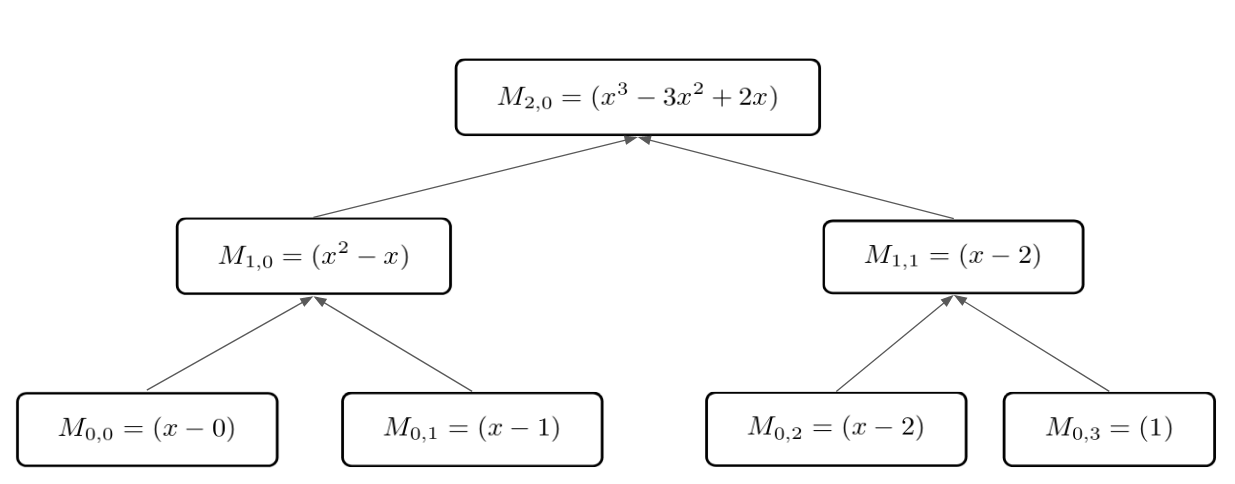
\includegraphics [scale=0.25]{bab2/img/pohon-polinomial-n-10}
	\caption {Pohon Polinomial untuk $ N  = 10 $}
	\label {fig:pohon-polinomial-n-10}
\end{figure}

\subsection{Evaluasi Pohon Polinomial}
\label{sec:evaluasi_pohon_polinomial}
Setelah pohon polinomial dibangun, langkah selanjutnya adalah mengevaluasi polinomial $ g(x) $ dengan \textit{Multipoint Evaluation}. Algoritma ini merupakan algoritma \textit{divide-and-conquer} yang menggunakan \textit{Chineese Remainder Theorem} sebagai dasar.
\begin{theo}[Teorema Sisa Polinomial]
	\label{theo:teorema_sisa_poli}
	Bentuk umum pembagian polinomial adalah $ F(x) = P(x) \cdot H(x) + S(x) $ \\
	$ F(x) $ = polinomial awal \\
	$ P(x) $ = polinomial pembagai \\
	$ H(x) $ = polinomial hasil bagi \\
	$ S(x) $ = polinomial sisa \\
	\begin{enumerate}
		\item Jika polinomial $ F(x) $ berderajat $ n $ dibagi oleh $ (x - k) $ maka sisanya adalah $ F(k) $.
		\item Jika polinomial $ F(x) $ berderajat $ n $ dibagi oleh $ (ax - b) $ maka sisanya adalah $ F(\frac{b}{a}) $.
		\item Jika polinomial $ F(x) $ berderajat $ n $ dibagi oleh $ (x - a)(x - b) $ maka sisanya adalah $ \frac{F(a) - F(b)}{a - b} +  \frac{aF(a) - bF(b)}{a - b}$.
	\end{enumerate}
\end{theo}
Pada teorema \ref{theo:teorema_sisa_poli}, sisa hasil bagi $ f $ dengan $ (x - u_i ) $ sama dengan hasil dari $ f(u_i) $ yaitu 
\begin{equation}
	\begin{aligned}
		f(u_i) &= q(u_i) \cdot m_i(u_i) + r(u_i) \\
			   &= q(u_i).0 + r(u_i) \\
			   &= r(u_i) \\
			   &= f \text{ mod } (x - u_i)
	\end{aligned}
	\label{eq:f_mod_ui}
\end{equation}

Persamaan \eqref{eq:f_mod_ui} merupakan dasar dari metode evaluasi polinomial pada $ n $ titik sehingga evaluasi dilakukan dengan membagi polinomial $ g(x) $ dengan $ n $ mono polinomial $ (x + u_i) $. Akan tetapi pembagian polinomial berderajat $ n-1 $ dengan $ n $ mono polinomial memiliki kompleksitas $ \mathcal{O}{(n^2)} $, sehingga akan menjadi \textit{bottleneck} dalam algoritma ini. Tetapi dengan pohon polinomial, pembagian polinomial $g(x)$ dapat dilakukan secara bertahap dengan setiap \textit{node} pada pohon polinomial. 
\begin{equation}
	\begin{aligned}
		r = f \text{ mod }  M_{k,0}
		\label{eq:nilai_awal_r}
	\end{aligned}
\end{equation}
Dimisalkan polinomial $ r $ memiliki nilai awal seperti pada persamaan \eqref{eq:nilai_awal_r}, dengan polinomial $ f $ merupakan input dari setiap \textit{node} pada pohon polinomial. Nilai $ f $ untuk akar dari pohon polinomial adalah polinomial $ g(x) $, sementara untuk \textit{node} lain adalah polinomial $ r $ yang didapatkan dari \textit{parent node}. Karena pohon polinomial merupakan pohon biner, maka jumlah pembagian polinomial untuk menghitung evaluasi berkurang dari $ \mathcal{O}{(n)} $ menjadi $ \mathcal{O}{(\text{log }n)} $. Untuk $ N = 10 $ maka proses evaluasi polinomial $ g(x) $ diilustrasikan seperti gambar \ref{fig:evaluasi-pohon-n-10}.

\begin{figure}
	\Centering
	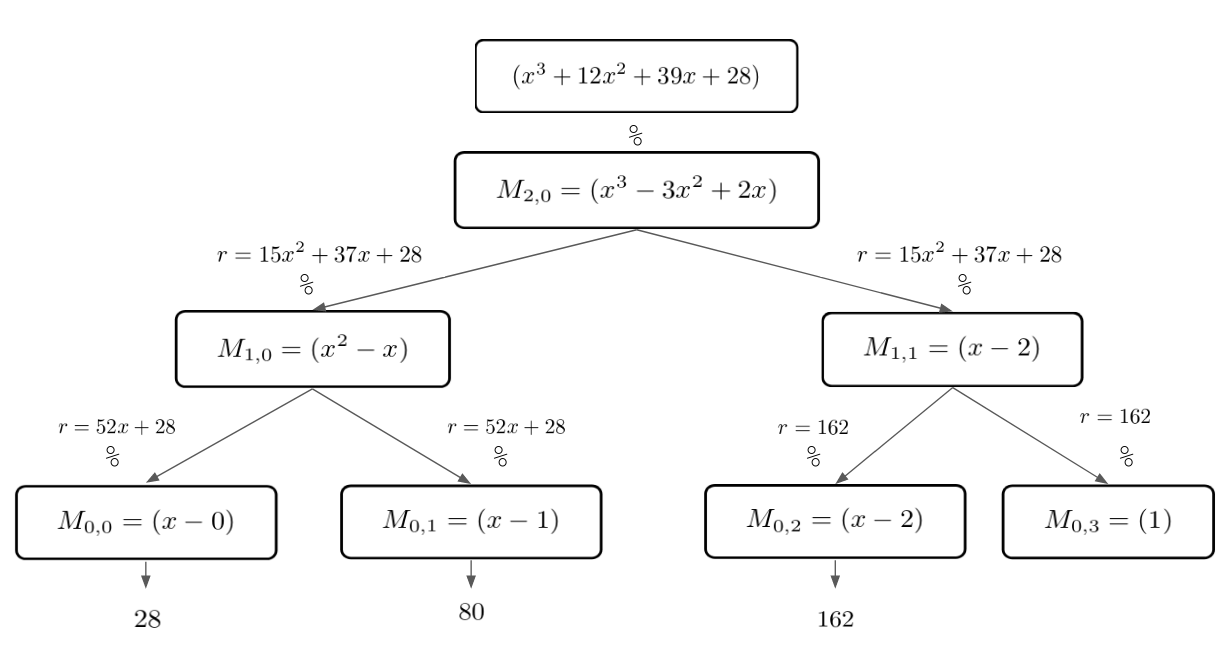
\includegraphics [scale=0.25]{bab2/img/evaluasi-pohon-n-10}
	\caption{Evaluasi pada Pohon Polinomial untuk $ N = 10 $}
	\label{fig:evaluasi-pohon-n-10}
\end{figure}

\begin{algorithm}
	\caption{Evaluasi Pohon Polinomial (General)}
	\label{psdo:general_evaluasi_pohon_polinomial}
	\begin{algorithmic}[1]
		\Require $ N = 2^k, k \in \mathbb{N},f \in R[x] \text{ dan pohon polinomial } M_{i,j}  $
		\Ensure $ f(u_0), \cdots , f(u_{n-1}) $
		\State $ r \gets f \text{ mod } M_{k,0} $
		\State panggil fungsi dengan input $ r, n/2 $ dan pohon dengan root $ M_{k-1,0} $
		\State panggil fungsi dengan input $ r, n/2 $ dan pohon dengan root $ M_{k-1,1} $ \\
		\Return $ r(u_0), \cdots , r(u_{n-1})) $
	\end{algorithmic}
\end{algorithm}

Pada pseudocode \ref{psdo:general_evaluasi_pohon_polinomial}, bagian yang memiliki kompleksitas paling tinggi adalah melakukan operasi $ f \mod{M_{i,j}} $ untuk setiap polinomial $ M_{i,j} $ dalam pohon polinomial. Algoritma ini berjalan secara rekursi, dengan membagi hasil operasi sekarang dengan node dibawahnya. Apabila $ D(n) \simeq 8M(n) $ merepresentasikan kompleksitas pembagian polinomial berderajat $ n - 1 $ dengan polinomial berderajat $ \frac{n}{2} $ yang berbasis \textit{Fast Fourier Transform}, maka kompleksitas perhitungan evaluasi pohon polinomial ditunjukan pada persamaan \eqref{eq:kompleksitas_evaluasi_pohon_polinomial}:
\begin{equation}
	\begin{aligned}
		T(n) &= 2T(\frac{n}{2}) + D(n) \\
			 &\leq 2T(\frac{n}{2}) + 8M(n) \\
			 &\leq \text{log}_2 n(8M(n)) \\
			 &\leq 8n\text{ log}^2 n \\
			 &\in \mathcal{O}{(n \text{ log}^2\ n)} \\
	\end{aligned}
	\label{eq:kompleksitas_evaluasi_pohon_polinomial}
\end{equation}

\subsection{Komputasi Faktorial berdasarkan Hasil Evaluasi}
\label{sec:komputasi_faktorial_multipoint}
Setelah mendapatkan nilai dari $ g(0), g(1), \cdots, g(v-1) $, langkah selanjutnya adalah menghitung nilai dari $ N! $. Mengulang dari subbab \ref{sec:perumusan_transformasi_faktorial} dan persamaan \eqref{eq:persamaan_faktorial_baru}, didapatkan persamaan faktorial baru sebagai berikut.
$$ N ! = \left( \prod_{i=0}^{v-1} g(i) \right) \cdot \prod_{i=v^2+1}^n i $$
Menggunakan teorema \ref{theo:wilson}, kompleksitas algoritma dapat diturunkan. Sebagai contoh, apabila $ N = 9 $ dan $ P = 13 $ maka 
\begin{equation}
	\begin{aligned}
	9! &\equiv \frac{-1}{12 \cdot 11 \cdot 10} \mod{13} \\
	   &\equiv \frac{-1}{-1 \cdot -2 \cdot -3} \mod{13} \\
	   &\equiv 11 \mod{13}. \\
	\end{aligned}
\end{equation}
\begin{theo}[Wilson's Theorem]
	\label{theo:wilson}
	Jika terdapat bilangan asli $ p > 1 $ adalah bilangan prima, maka hasil perkalian dari semua bilangan bulat positif yang kurang dari n ditambah 1 adalah kelipatan dari $ p $. Sehingga dalam notasi kongruen dapat didefinisikan persamaan \eqref{eq:wilson_theorem}.
	\begin{equation}
		(p - 1)! \equiv -1 \Mod{p}
		\label{eq:wilson_theorem}
	\end{equation}
\end{theo}
Sehingga persamaan \eqref{eq:persamaan_faktorial_baru}, dapat diubah menjadi persamaan \eqref{eq:rumus_faktorial_baru2}
$$ \text{faktorial}(n) = \left( \prod_{i=0}^{v-1} g(i) \right) \cdot \prod_{i=v^2+1}^n i $$
\begin{equation}
	N! \equiv
	\begin{cases}
		\text{faktorial}(N), 	      & \text{jika } 2N < P \\\\
		\dfrac{1}{\text{faktorial}(M)}
		& \text{jika } 2N >= P \text{ dan } M \text{ genap}\\\\
		P -\dfrac{1}{\text{faktorial}(M)}
		& \text{jika } 2N >= P \text{ dan } M \text{ ganjil} \\
	\end{cases}
	\label{eq:rumus_faktorial_baru2}
\end{equation}
$$ \text{ dengan } M = P-N-1 $$

Karena derajat polinomial terbesar pada algoritma ini adalah $ p = \sqrt{\frac{P}{2}} $, dengan mengingat kompleksitas dari pembangunan pohon faktorial \eqref{eq:kompleksitas_pohon_polinomial} dan evaluasi pohon faktorial \eqref{eq:kompleksitas_evaluasi_pohon_polinomial} maka kompleksitas total perhitungan faktorial menggunakan \textit{Multipoint Evaluation} adalah :
\begin{equation}
	\begin{aligned}
		&= \mathcal{O}{(p \text{ log}^2\ p)} + \mathcal{O}{(p \text{ log}^2\ p)} + \mathcal{O}{(p)} \\
		&\leq \mathcal{O}{(2p \text{ log}^2\ p)} + \mathcal{O}{(p)} \\
		&\leq \mathcal{O}{(2p \text{ log}^2\ p)} \\
		&\in \mathcal{O}{(p \text{ log}^2\ p)} \\
	\end{aligned}
	\label{eq:kompleksitas_multipoint_eval_faktorial}
\end{equation}

\newpage

\section{Strategi Penyelesaian dengan Shifting Evaluation Values}
Pada subbab ini akan dipaparkan mengenai strategi penyelesaian masalah klasik pada daring SPOJ dengan kode FACTMODP menggunakan \textit{Shifting Evaluation Values}. Secara singkat, strategi penyelesaian masalah dari FACTMODP menggunakan \textit{Shifting Evaluation Values} terbagi menjadi 3 bagian besar yaitu :
\begin{enumerate}
	\item Shifting Evaluation Values
	\item Implementasi Shiting Evaluasi Values pada Perhitungan Faktorial
	\item Komputasi Faktorial berdasarkan Hasil Evaluasi
\end{enumerate}

Sebagai contoh, pada subbab ini akan menggunakan $ N = 17 $ serta $ P = 10^9 + 7 $ sebagai modulo. Nilai $ N $ dan $ P $ yang dipilih berada didalam batasan yang didefinisikan dalam subbab \ref{sec:batasan_masalah}. Persoalan utama dalam Tugas Akhir ini adalah memodelkan faktorial sedemikian hingga dapat dikomputasi dengan kompleksitas dibawah $ \mathcal{O}{(N)} $.

\subsection{Shifting Evaluation Values}
Pada subbab ini akan dibahas mengenai algoritma \textit{Shifting Evaluation Values} secara umum. Pada subbab \ref{sec:penyelesaian_multipoint_evaluation}, dikatakan bahwa polinomial $ g(x) $ dievaluasi pada $ 0, 1, \cdots, v-1 $, sehingga membentuk deret aritmatika. Pseudocode \ref{psdo:shifting_evaluation_values} menjelaskan bagaimana secara umum algoritma \textit{Shifting Evaluation Values} bekerja dalam $ \mathbb{R} $. Dimisalkan $ a $ dan $ r_0, r_1, \cdots, r_d $ merupakan titik dalam $ \mathbb{R} $, sehingga diketahui nilai dari $$ P(r_0), P(r_1), \cdots, P(r_d) $$ maka \textit{Shifting Evaluation Values} menghitung nilai dari $$ P(r_0 + a), P(r_1 + a), \cdots, P(r_d + a) $$ dengan kompleksitas $ \mathcal{M}{(2d)} + \mathcal{O}{(d)} $.
\begin{algorithm}
	\caption{Shifting Evaluation Values (General)}
	\label{psdo:shifting_evaluation_values}
	\begin{algorithmic}[1]
		\Require $ P(0), \cdots. P(d) \text{ dan } a \in \mathbb{R} $
		\Ensure $ P(a), \cdots , P(a+d) $
		\State $ \delta(0,d) = \prod_{j=1}^d(-j) $
		\State $ \delta(i,d) = \frac{i}{i - d - 1} \delta(i-1,d)\ \ i = 1, \cdots, d$
		\State $ \Delta(a,0,d) = \prod_{j=1}^d(a-j) $
		\State $ \Delta(a,k,d) = \frac{a+k}{a+k - d - 1} \Delta(a,i-1,d)\ \ k = 1, \cdots, d $
		\State $ \tilde{P} = \sum_{i=0}^d \frac{P(i)}{\delta(i,d)} X^i $ 
		\State $ S = \sum_{i=0}^{2d} \frac{1}{a + i - d} X^i,$ 
		\State $ Q = \tilde{P}S. $ \\ 
		\Return $ \Delta(a,0,d)\cdot \texttt{coef}(Q,d), \cdots, $ $ \Delta(a,d,d)\cdot \texttt{coef}(Q,2d)  $
	\end{algorithmic}
\end{algorithm}

Penulis menggunakan notasi $ \texttt{coef}(Q,k) $ pada pseudocode \ref{psdo:shifting_evaluation_values} untuk merepresentasikan koefisien dari derajat ke-$k$ dari polinomial $Q$. Pseudocode \ref{psdo:shifting_evaluation_values} juga menjelaskan bahwa polinomial $ g(x) $ tidak menjadi input dari algoritma ini.

\begin{theo}[Teorema Shifting Evaluation Values]
	\label{theo:shifting_evaluation_values}
	Dimisalkan $ \mathbb{R} $ adalah ring komutatif dan $ d \in \mathbb{N} $  sehingga $ 1, \cdots, d $ adalah unit dalam $ \mathbb{R} $. $ P $ merupakan polinomial dengan derajat $ d $, sehingga barisan 
	$$ P(0), \cdots. P(d) $$
	diketahui. Dimisalkan $ a $ juga berada dalam  $ \mathbb{R} $, sehingga $ a-d, \cdots, a+d $ adalah unit dalam $ \mathbb{R} $ sehingga barisan 
	$$ P(a), \cdots. P(a+d) $$
	bisa dihitung dengan kompleksitas waktu $ M(2d) + O(d) $ dan menggunakan ruang $ O(d) $.
\end{theo}

Pembuktian mengenai teorema \ref{theo:shifting_evaluation_values} didasari dengan persamaan \eqref{eq:interpolasi_lagrange} yang disebut interpolasi \textit{Lagrange} sebagai berikut
\begin{equation}
	\label{eq:interpolasi_lagrange}
	P = \sum_{i=0}^d P(i) \frac{\prod_{j=0, j \neq i}^d (X-j)}{\prod_{j=0, j \neq i}^d (i-j)}.
\end{equation}
Apabila $ \delta(i,d) = \prod_{j=0, j \neq i}^d (i-j) $ serta $  \tilde{P_i} = \frac{P(i)}{\delta(i,d)} $ maka melalui pseudocode \ref{psdo:shifting_evaluation_values}, dapat disimpulkan bahwa perhitungan nilai $ \delta(i,d) $ dapat dihitung dalam $ \mathcal{O}{(d)} $. Meskipun perhitungan $ \delta(0,d) $ memerlukan $ d $ perkalian, tetapi untuk $ i = 1, 2, \cdots, d $, nilai $\delta(i,d) $ dapat dihitung dengan menggunakan persamaan rekursi \eqref{eq:rekursi_delta_kecil}.
\begin{equation}
	\delta(i,d) = \frac{i}{i - d - 1} \delta(i-1,d).
	\label{eq:rekursi_delta_kecil}
\end{equation}
Sehingga persamaan \eqref{eq:interpolasi_lagrange}, dapat ditulis kembali menjadi persamaan \eqref{eq:interpolasi_lagrange_2}
\begin{equation}
	P = \sum_{i=0}^d \tilde{P_i} \prod_{j=0, j \neq i}^d (X-j)
	\label{eq:interpolasi_lagrange_2}
\end{equation}
Untuk $ k \text{ dari } 0, 1, \cdots, d $, maka evaluasi $ P $ pada titik $ a + k $ ditunjukan pada persamaan \eqref{eq:interpolasi_lagrange_3}.
\begin{equation}
	P(a+k) = \sum_{i=0}^d \tilde{P_i} \prod_{j=0, j \neq i}^d (a+k-j)
	\label{eq:interpolasi_lagrange_3}
\end{equation}
Persamaan \eqref{eq:interpolasi_lagrange_3}, dapat disederhanakan menjadi persamaan \eqref{eq:interpolasi_langrange_4}.
\begin{equation}
	\begin{aligned}
	P(a+k)  &= \sum_{i=0}^d P(i) \frac{\prod_{j=0, j \neq i}^d (a+k-j)}{\prod_{j=0, j \neq i}^d (i-j)} \\
			&= \sum_{i=0}^d P(i) \cdot \prod_{j=0}^{d} a+k-j \cdot \frac{1}{a + k - i} \cdot \prod_{j=0, j\neq i}^d \frac{1}{i-j} \\
			&= \left( \prod_{j=0}^d a+k-j \right) \left( \sum_{i=0}^d P(i) \cdot  \cdot \frac{1}{a + k - i} \cdot \prod_{j=0, j\neq i}^d \frac{1}{i-j} \right) \\
			&= \left( \prod_{j=0}^d a+k-j \right) \cdot \left( \sum_{i=0}^d P(i) \cdot \frac{1}{a + k - i} \cdot \frac{1}{i! (d-i)! (-1)^{d-1}} \right) \\
			&= \left( \prod_{j=0}^d a+k-j \right) \cdot \left( \sum_{i=0}^d \frac{P(i)}{i! (d-i)! (-1)^{d-1}} \cdot \frac{1}{a + k - i} \right) \\
	\end{aligned}
	\label{eq:interpolasi_langrange_4}
\end{equation}
Apabila  $ \Delta (a,k,d) = \prod_{j=0}^d (a+k-j) $, sama dengan $ \delta(i,d) $, perhitunga $ \Delta(a,k,d), \text{ untuk }k = 0, 1, \cdots, d $ dapat dihitung dengan kompleksitas $ \mathcal{O}{(d)} $ menggunakan persamaan \eqref{eq:rekursi_delta_besar}.
\begin{equation}
	\begin{aligned}
		\Delta (a,0,d) &= \prod_{j=1}^d(a-j) \\
		\Delta(a,k,d) &= \frac{a+k}{a+k - d - 1} \Delta(a,k-1,d)\ \ k = 1, 2, \cdots, d
	\end{aligned}
	\label{eq:rekursi_delta_besar}
\end{equation}
Apabila polinomial $ \tilde{P} \text{ dan } S $ memiliki nilai seperti pada persamaan \eqref{eq:P_dan_S}
\begin{equation}
	\tilde{P} = \sum_{i=0}^d \tilde{P_i} X^i , S = \sum_{i=0}^{2d} \frac{1}{a+i-d} X^i
	\label{eq:P_dan_S}
\end{equation}
untuk $ k=0, \cdots, d$ , maka $ \sum_{i=0}^d \tilde{P_i} \frac{1}{a+k-i} $ adalah koefisien dengan derajat $ k+d $ dalam polinomial $ \tilde{P}S $, sehingga teorema terbukti.

Fungsi pada pseudocode \ref{psdo:shifting_evaluation_values} hanya mengembalikan \textit{middle product} dari perkalian polinomial $ Q = \tilde{P}S $. Untuk menghitung \textit{middle product}, dapat menggunakan algoritma bernama \textit{Middle Product Optimization}.\textit{ Midlle Product Optimization} merupakan teknik optimasi dalam menemukan \textit{middle product} dari perkalian polinomial $ A , B $ dengan derajat $ d $ dan $ 2d $, sehingga $$ AB = C_0 + C_1X^{d+1} + C_2X^{2d+2}. $$ $ C_1 $ disebut sebagai \textit{midlle product} dari $ AB $. Pada subbab berikutnya akan dijelaskan mengenai algoritma \textit{midlle product optimization} lebih lengkapnya. 
% TODO : subbab berapaahh

\subsection{Implementasi Shifting Evaluation Values pada Perhitungan Faktorial}

\begin{figure}
	\Centering
	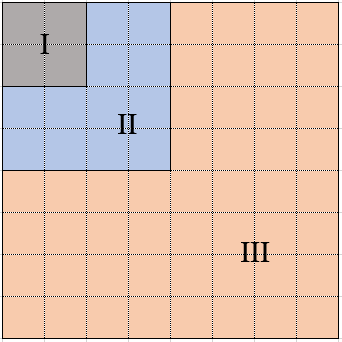
\includegraphics [scale=0.6]{bab2/img/kotak-pembagian-daerah}
	\caption {Pembagian daerah \textit{\textit{grid}}}
	\label {fig:kotak-pembagian-daerah}
\end{figure}

Untuk memvisualisasikan implementasi ini, maka didefinisikan \textit{\textit{grid}} berukuran $ v \times v $ beserta level pada \textit{\textit{grid}} seperti pada gambar \ref{fig:kotak-pembagian-daerah}. Dimisalkan bilangan bulat positif $ v = \lfloor \sqrt{N} \rfloor $, polinomial $ f(x) $ dan bilangan bulat $ x_1 $ sehingga $ f(x_1) = 1 \text{ dan } f(x_1+1) = v+1 $. Tujuan akhir dalam subbab ini adalah menghasilkan \textit{\textit{grid}} dengan ukuran $ v \times v $ sebagai berikut menggunakan \textit{Shifting Evaluation Values}.

\begin{table}[H]
	\centering
	\begin{tabular}{|c|c|c|c|} \hline
	1  & 2  & 3  & 4  \\ \hline
	5  & 6  & 7  & 8  \\ \hline
	9  & 10 & 11 & 12 \\ \hline
	13 & 14 & 15 & 16 \\ \hline
	\end{tabular}
\end{table}

Pada awalnya, terdapat nilai awal pada \textit{\textit{grid}}, $ 1 , 5 $ melambangkan nilai dari $ f(x_1) \text{ dan } f(x_1 + 1) $ secara berurutan. 
\begin{table}[H]
	\centering
	\begin{tabular}{|c|c|c|c|} \hline
	1  & $ R_{1,2} $ & $ R_{1,3} $ & $ R_{1,4} $ \\ \hline
	5  & $ R_{2,2} $ & $ R_{2,3} $ & $ R_{2,4} $ \\ \hline
	$ R_{3,1} $  & $ R_{3,2} $ & $ R_{3,3} $ & $ R_{3,4} $ \\ \hline
	$ R_{4,1} $  & $ R_{4,2} $ & $ R_{4,3} $ & $ R_{4,4} $ \\ \hline
	\end{tabular}
\end{table}
Langkah pertama adalah mengisi $ R_{1,2} $ dan $ R_{2,2} $ untuk melengkapi daerah level I menggunakan algoritma \textit{Shifting Evaluation Values}. Menggunakan pseudocode \ref{psdo:shifting_evaluation_values} dengan input $ a = \frac{1}{v} $, maka nilai $ R_{1,2} $ dan $ R_{2,2} $ adalah $ 2 $ dan $ 6 $. 

Pada level II, \textit{grid} sebelumnya diubah menjadi \textit{grid} baru dengan mengalikan nilai dari 2 kolom, yaitu kolom 1 dengan kolom 2 dan kolom 3 dengan kolom 4.
\begin{table}[H]
	\centering
	\begin{tabular}{|c|c|c|c|} \hline
	$ 1  \times 2 $ & $ R_{1,3} \times R_{1,4} $ \\ \hline
	$ 5  \times 6 $ & $ R_{2,3} \times R_{2,4} $ \\ \hline
	$ R_{3,1} \times R_{3,2} $ & $ R_{3,3} \times R_{3,4} $ \\ \hline
	$ R_{4,1} \times R_{4,2} $ & $ R_{4,3} \times R_{4,4} $ \\ \hline
	\end{tabular}
\end{table}
Didefinisikan array $ P = \{1 \times 2, 5 \times 6 \}$, menggunakan pseudocode \ref{psdo:shifting_evaluation_values} dengan input $ P $ dan $ a = \frac{2}{v} $, maka akan didapatkan nilai dari $ R_{1,3} \times R_{1,4} $ dan $ R_{2,3} \times R_{2,4} $ yaitu $ 12 \text{ }(3 \times 4) $ dan $ 56 \text{ } (7 \times 8) $.

Dengan menggunakan langkah yang sama, tetapi dengan input $ a = \frac{v}{v} $ dan $ a = \frac{v+2}{v} $, maka akan didapatkan nilai dari $ R_{3,1} \times R_{3,2} $, $ R_{4,1} \times R_{4,2} $, $ R_{3,3} \times R_{3,4} $ , dan $ R_{4,3} \times R_{4,4} $ adalah $ 90 \text{ } (9 \times 10) $ , $ 182 \text{ } ( 13 \times 14) $, $ 132 \text{ } (11 \times 12) $ dan $ 240 \text{ } ( 15 \times 16) $.

% Dengan langkah yang sama tetapi dengan input $ a = \frac{v}{v} $, maka akan didapatkan nilai dari $ R_{3,1} \times R_{3,2} $ dan $ R_{4,1} \times R_{4,2} $ yaitu $ 90 \text{ } (9 \times 10) $ dan $ 182 \text{ } ( 13 \times 14) $, 

% Dengan langkah yang sama tetapi dengan input $ a = \frac{v+2}{v} $, maka akan didapatkan nilai dari $ R_{3,3} \times R_{3,4} $ dan $ R_{4,3} \times R_{4,4} $ yaitu $ 132 \text{ } (11 \times 12) $ dan $ 240 \text{ } ( 15 \times 16) $.

Pada akhir level II, \textit{grid} memiliki nilai sebagai berikut
\begin{table}[H]
	\centering
	\begin{tabular}{|c|c|c|c|} \hline
	$ 1  \times 2 $ & $ 3 \times 4 $ \\ \hline
	$ 5  \times 6 $ & $ 7 \times 8 $ \\ \hline
	$ 9  \times 10 $ & $ 11 \times 12 $ \\ \hline
	$ 13 \times 14 $ & $ 15 \times 16 $ \\ \hline
	\end{tabular}
\end{table}

Selanjutnya adalah level III, pada level III, \textit{grid} diubah menjadi \textit{grid} baru dengan mengalikan nilai dari 2 kolom, yaitu kolom 1 dengan kolom 2.
\begin{table}[H]
	\centering
	\begin{tabular}{|c|c|c|c|} \hline
	$ 1  \times 2 \times 3 \times 4  = 24 $ \\ \hline
	$ 5  \times 6 \times 7 \times 8  = 1680 $ \\ \hline
	$ 9  \times 10 \times 11 \times 12  = 11880 $ \\ \hline
	$ 13 \times 14 \times 15 \times 16  = 43680 $ \\ \hline
	\end{tabular}
\end{table}
Tetapi karena \textit{grid} tersebut sudah tidak memiliki nilai kosong, maka proses implementasi \textit{Shifting Evaluation Values} sudah selesai. Pada setiap level, diperlukan 3 kali proses \textit{Shifting Evaluation Values}, dan untuk keseluruhan proses diperlukan $ \text{log}_2 (v) $ level. Apabila $ M(n) \simeq \mathcal{O}{(n \text{ log } n)} $ merepresentasikan kompleksitas perkalian polinomial berbasis \textit{Fast Fourier Transform} dengan derajat kurang dari $ n $ dan $ 0 \leq m < k $ maka kompleksitas yang dibutuhkan untuk membangun grid ditunjukan oleh persamaan \eqref{eq:kompleksitas_grid}.
\begin{equation}
	\begin{aligned}
			 &\leq \text{log}_2 (3 \times (M(2n) + O(n))) \\
			 &\leq 6n\text{ log}^2 n \\
			 &\in \mathcal{O}{(n \text{ log}^2\ n)} \\
	\end{aligned}
	\label{eq:kompleksitas_grid}.
\end{equation}

\subsection{Komputasi Faktorial berdasarkan Hasil Evaluasi}
Setelah \textit{grid} sudah tidak memiliki nilai kosong, didefinisikan \textit{array} $ G $ berukuran $ 1 \times v $, dengan nilai $ \{ row_1, row_2, \cdots, row_3 \} $, dimana $ row_i $ menyatakan nilai dari baris ke-$i$ dari \textit{grid} yang sudah dihitung sebelumnya. Maka didefinisikan rumus faktorial baru untuk \textit{Shifting Evaluation Values} seperti pada persamaan \eqref{eq:persamaan_faktorial_baru_2}
\begin{equation}
	N! = \text{faktorial}(n) = \left( \prod_{i=0}^{v-1} G(i) \right) \cdot \prod_{i=v^2+1}^n i
	\label{eq:persamaan_faktorial_baru_2}
\end{equation}

Sama seperti subbab \ref{sec:komputasi_faktorial_multipoint}, menggunakan teorema \ref{theo:wilson}, kompleksitas perhitungan faktorial dapat diturunkan, sehingga persamaan \eqref{eq:persamaan_faktorial_baru_2}, dapat diubah menjadi persamaan \eqref{eq:persamaan_faktorial_baru_3}.
$$ \text{faktorial}(n) = \left( \prod_{i=0}^{v-1} G(i) \right) \cdot \prod_{i=v^2+1}^n i $$
\begin{equation}
	N! \equiv
	\begin{cases}
		\text{faktorial}(N), 	      & \text{jika } 2N < P \\\\
		\dfrac{1}{\text{faktorial}(M)}
		& \text{jika } 2N >= P \text{ dan } M \text{ genap}\\\\
		P -\dfrac{1}{\text{faktorial}(M)}
		& \text{jika } 2N >= P \text{ dan } M \text{ ganjil} \\
	\end{cases}
	\label{eq:persamaan_faktorial_baru_3}
\end{equation}
$$ \text{ dengan } M = P-N-1 $$

Karena derajat polinomial terbesar pada algoritma ini adalah $ p = \sqrt{\frac{P}{2}} $, dengan mengingat kompleksitas dari perhitungan grid \eqref{eq:kompleksitas_grid}, maka kompleksitas total perhitungan faktorial menggunakan \textit{Shifting Evaluation Values} adalah :
\begin{equation}
	\begin{aligned}
		&= \mathcal{O}{(p \text{ log}^2\ p)} + \mathcal{O}{(p)} \\
		&\in \mathcal{O}{(p \text{ log}^2\ p)} \\
	\end{aligned}
	\label{eq:kompleksitas_shifting_eval_faktorial}
\end{equation}

\section{Strategi Penyelesaian Operasi Polinomial}
Pada subbab ini akan dipaparkan mengenai strategi penyelesaian operasi polinomial yang sering digunakan dalam dua algoritma yang dibahas pada subbab sebelumnya. Secara singkat, strategi penyelesaian operasi polinomial terbagi menjadi 3 bagian besar yaitu :
\begin{enumerate}
	\item Penjumlahan dan Pengurangan Polinomial
	\item Perkalian Polinomial
	\item Pembagian Polinomial
\end{enumerate}

\subsection{Penjumlahan dan Pengurangan Polinomial}
Polinomial juga bisa diterapkan operasi pertambahan dan pengurangan dalam aritmatika. 
Didefinisikan 2 buah polinomial $f(x)$ dan $g(x)$ sebagai berikut.
$$ f(x) = a_n x^n + a_{n-1}^{n-1} + \cdots + a_2x^2 + a_1x + a_0 $$
$$ g(x) = b_m x^m + b_{m-1}^{m-1} + \cdots + b_2x^2 + b_1x + b_0 $$
Pada umumya operasi pertambahan polinomial $ f(x) + g(x) $ dinyatakan seperti dalam persamaan \eqref{eq:persamaan_tambah_polinomial}.
\begin{equation}
	f(x) + g(x) = \sum_{i=0}^{max(n,m)} (a_i + b_i) x^i
	\label{eq:persamaan_tambah_polinomial} 
\end{equation}
Kemudian operasi pengurangan polinomial $ f(x) - g(x) $ dinyatakan seperti dalam persamaan \eqref{eq:persamaan_kurang_polinomial}.
\begin{equation}
	f(x) - g(x) = \sum_{i=0}^{max(n,m)} (a_i - b_i) x^i
	\label{eq:persamaan_kurang_polinomial} 
\end{equation}
Secara umum kompleksitas operasi pertambahan dan pengurangan dari polinomial adalah $ \mathcal{O}{(max(n,m))} $ dengan $ n , m $ adalah derajat polinomial $ f(x) \text{ dan } g(x) $.

\subsection{Perkalian Polinomial}
Selain pertambahan dan pengurangan, polinomial juga terdapat operasi perkalian.
Didefinisikan 2 buah polinomial $f(x)$ dan $g(x)$ sebagai berikut.
$$ f(x) = a_n x^n + a_{n-1}^{n-1} + \cdots + a_2x^2 + a_1x + a_0 $$
$$ g(x) = b_m x^m + b_{m-1}^{m-1} + \cdots + b_2x^2 + b_1x + b_0 $$
Pada umumnya operasi perkalian polinomial $ f(x) \cdot g(x) $ dinyatakan seperti dalam persamaan \eqref{eq:persamaan_kali_polinomial}.
\begin{equation}
	f(x) \cdot g(x) = \sum_{i=0}^{n} \sum_{j=0}^{m} (a_i \times b_j) x^{i+j}
	\label{eq:persamaan_kali_polinomial}
\end{equation}
Secara umum kompleksitas operasi perkalian polinomial adalah $ \mathcal{O}{(nm)} $ dengan $ n , m $ adalah derajat polinomial $ f(x) \text{ dan } g(x) $. Kompleksitas operasi perkalian ini dapat dikurangi menggunakan FFT atau \textit{Fast Fourier Transform}.

\subsubsection{Fast Fourier Transform}
Pada tahun 1965, James W. Cooley dan John W. Tukey berhasil merumuskan suatu teknik perhitungan algoritma \textit{Fourier Transform} yang efisien\cite{fft}. Teknik perhitungan algoritma ini dikenal dengan sebutan \textit{Fast Fourier Transform} atau lebih populer dengan istilah FFT. \textit{Fast Fourier Transform} dalam bahasa indonesia adalah Transformasi Fourier Cepat adalah sumber dari suatu algoritma untuk menghitung \textit{Discrete Fourier Transform (DFT)} atau Transformasi Fourier Diskrit dengan cepat dan efisien beserta dengan inversenya.

Transformasi Fourier Cepat diterapkan dalam berbagai bidang mulai dari pengolahan signal digital, memecahkan persamaan differensial parsial, sampai dalam perkalian polinomial. Terdapat dua pendekatan dari algoritma FFT yaitu \textit{Decimation in Time (DIT)} dan \textit{Decimation in Frequency (DIF)}. Pada subbab ini akan dijelaskan FFT yang digunakan untuk perkalian polinomial dengan pendekatan \textit{Decimation in Time (DIT)}.

Pada umumnya, dalam perkalian polinomial, FFT melakukan 3 tahapan sebagai berikut :
\begin{enumerate}
	\item Mengevaluasi polinomial $ f(x) $ dan $ g(x) $ pada banyak titik $ x_m $
	\item Mencari nilai titik baru dari perkalian $ f(x_m) \cdot g(x_m) $
	\item Mencari polinomial yang melalui titik-titik tersebut.
\end{enumerate}
Pencarian polinomial yang melalui titik-titik perkalian $ f(x_m) \cdot g(x_m) $, dapat menggunakan interpolasi langrange, tetapi karena kompleksitasnya yang besar, sehingga diperlukan pendekatan lain. Disinilah Transformasi Fourier Diskrit (DFT) berperan, dalam DFT apabila ingin mengalikan 2 polinomial dengan derajat maksimal $ n $, maka diperlukan $ n $ nilai dari $ x_m $ sebagai $n$\textit{-th roots of unity}. Persamaan untuk $n$\textit{-th roots of unity} dapat dilihat pada persamaan \eqref{eq:nth_root_of_unity}.
\begin{equation}
	\omega_n = \exp(\frac{-2\pi i}{n}) , x_m = \omega^m, 0 \leq m \leq n
	\label{eq:nth_root_of_unity}
\end{equation}
\textit{Roots of unity} adalah $ n $ bilangan kompleks yang memenuhi persamaan $ z^{n} = 1 $. Pencarian nilai $ \omega_n $ dapat diselesaikan menggunakan persamaan trigonometri \eqref{eq:trigo_root_of_unity}.
\begin{equation}
	\omega_n = \exp(\frac{2\pi i}{n}) = \cos(\frac{2\pi}{n}) + i \sin(\frac{2\pi}{n})
	\label{eq:trigo_root_of_unity}
\end{equation}
\textit{Roots of unity} akan menjadi pilihan titik-titik yang dijadikan dasar pada evaluasi polinomial. \textit{Roots of unity} juga memiliki properti khusus seperti pada persamaan \eqref{eq:identitas_root_of_unity}.
\begin{equation}
	\begin{aligned}
		\omega_{N}^{N} = 1 \\
		\omega_{N}^{N+k} = \omega_{N}^{k} \\
		\omega_{N}^{N/2} = -1 \\
		\omega_{N}^{N/2+k} = -\omega_{N}^{k} \\
	\end{aligned}
	\label{eq:identitas_root_of_unity}
\end{equation}

Dengan menggunakan persamaan \eqref{eq:identitas_root_of_unity}, polinomial $ f(x) = a_0 + a_1x + .... a_7x^7 $ dapat di evaluasi dengan $8$\textit{-th roots of unity}
\begin{equation}
	\begin{aligned}
		f(\omega^0) = a_0 + a_1 \ \ \   + a_2\ \ \ \ \ + a_3\ \ \ \ \ + a_4\ \ \ \ \ + a_5\ \ \ \ \ + a_6\ \ \ \ \ + a_7  \ \ \ \ \\ 
		f(\omega^1) = a_0 + a_1\omega^1 + a_2\omega^2 + a_3\omega^3 + a_4\omega^4 + a_5\omega^5 + a_6\omega^6 + a_7\omega^7 \\ 
		f(\omega^2) = a_0 + a_1\omega^2 + a_2\omega^4 + a_3\omega^6 + a_4\ \ \ \ \ + a_5\omega^2 + a_6\omega^4 + a_7\omega^6 \\ 
		f(\omega^3) = a_0 + a_1\omega^3 + a_2\omega^6 + a_3\omega^1 + a_4\omega^4 + a_5\omega^7 + a_6\omega^2 + a_7\omega^5 \\ 
		f(\omega^4) = a_0 + a_1\omega^4 + a_2\ \ \ \  + a_3\omega^4 + a_4\ \ \ \  + a_5\omega^4 + a_6\ \ \ \ \ + a_7\omega^4 \\ 
		f(\omega^5) = a_0 + a_1\omega^5 + a_2\omega^2 + a_3\omega^7 + a_4\omega^4 + a_5\omega^1 + a_6\omega^6 + a_7\omega^3 \\ 
		f(\omega^6) = a_0 + a_1\omega^6 + a_2\omega^4 + a_3\omega^2 + a_4\ \ \ \ \ + a_5\omega^6 + a_6\omega^4 + a_7\omega^2 \\ 
		f(\omega^7) = a_0 + a_1\omega^7 + a_2\omega^6 + a_3\omega^5 + a_4\omega^4 + a_5\omega^3 + a_6\omega^2 + a_7\omega^1 \\ 
	\end{aligned}
	\label{eq:evaluasi_fft}
\end{equation}

Setelah mengevaluasi polinomial $ f $ dengan $8$\textit{-th roots of unity}, dengan menggunakan \textit{Decimation in Time (DIT)}, maka persamaan dapat dipecah menjadi dua bagian yaitu sampel dengan waktu ganjil dan genap menjadi persamaan \eqref{eq:fft_ordering_1}. Pemecahan persamaan ini memiliki beberapa metode, seperti metode ganjil-genap yang penulis gunakan dalam contoh maupun metode \textit{bit-reverse-index}. 
\begin{equation}
	X_k = \sum_{n=0}^{\frac{N}{2}-1} x_{2n}\omega_{N}^{2kn} + \omega_N^r \sum_{n=0}^{\frac{N}{2}-1} x_{2n+1}\omega_{N}^{2kn}
	\label{eq:fft_ordering_1}
\end{equation}
Menggunakan identitas \textit{roots of unity} pada persamaan \eqref{eq:identitas_root_of_unity}, maka persamaan \eqref{eq:fft_ordering_1} diubah menjadi persamaan \eqref{eq:fft_ordering_rumus}.
\begin{equation}
	X_k = \sum_{n=0}^{\frac{N}{2}-1} x_{2n}\omega_{\frac{N}{2}}^{kn} + \sum_{n=0}^{\frac{N}{2}-1} x_{2n+1}\omega_{\frac{N}{2}}^{kn}
	\label{eq:fft_ordering_rumus}
\end{equation}
Apabila dimisalkan $ y_n = x_{2n} $ dan $ x_n = x_{2n+1} $, maka persamaan \eqref{eq:fft_ordering_rumus} diubah menjadi persamaan \eqref{eq:fft-kiri} dan \eqref{eq:fft-kanan}.
\begin{equation}
	Y_k = \sum_{n=0}^{\frac{N}{2}-1} y_{n}\omega_{\frac{N}{2}}^{kn}
	\label{eq:fft-kiri}
\end{equation}
\begin{equation}
	Z_k = \sum_{n=0}^{\frac{N}{2}-1} z_{n}\omega_{\frac{N}{2}}^{kn}
	\label{eq:fft-kanan}
\end{equation}
Ketika persamaan \eqref{eq:fft-kiri} dan \eqref{eq:fft-kanan} diselesaikan secara rekursif, didapatkan setengah suku awal sama dengan persamaan \eqref{eq:kupu-kupu-1}. Dengan menggunakan identitas \textit{roots of unity} pada persamaan \eqref{eq:identitas_root_of_unity}, maka sisa setengah suku akhir ditunjukan pada persamaan \eqref{eq:kupu-kupu-2}.
\begin{equation}
	X_k = Y_k + \omega_{N}^{k} Z_k,\ k = 0,1,2,3 \cdots , \frac{N}{2}-1
	\label{eq:kupu-kupu-1}
\end{equation}
\begin{equation}
	X_{k+\frac{N}{2}} = Y_k - \omega_{N}^{k} Z_k,\ k = 0,1,2,3 \cdots , \frac{N}{2}-1
	\label{eq:kupu-kupu-2}
\end{equation}
Proses perhitungan dari persamaan \eqref{eq:kupu-kupu-1} dan \eqref{eq:kupu-kupu-2} merupakan operasi yang disebut dengan \textit{FFT Butterfly Cooley-Tukey} atau \textit{FFT Butterfly}. Skema \textit{FFT Butterfly} dengan metode pemecahan persamaan \textit{bit-reverse-index} ditunjukan pada gambar \ref{fig:bit-reverse-fft-butterfly}.

\subsubsection{Inverse Fast Fourier Transform} Inverse Fast Fourier Transform merupakan metode untuk mengembalikan hasil dari transformasi fourier cepat pada domain frekuensi menjadi domain waktu kembali, sehingga proses ini akan menghasilkan deret bilangan kompleks pada domain waktu kembali. Pada perkalian polinomial, inversi dari transformasi fourier dilakukan untuk merubah representasi titik dari polinomial setelah dilakukan perkalian secara $ \mathcal{O}{(N)} $ menjadi bentuk polinomial dengan representasi koefisien kembali. Transformasi inverse pada polinomial $ f(x) $ dilakukan menurut transformasi yang ditunjukan pada gambar \ref{fig:inverse-fft}.
\begin{figure}
	\Centering
	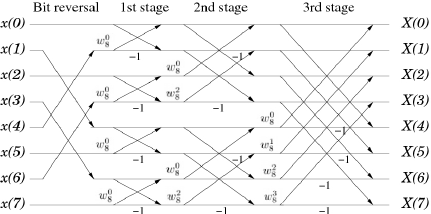
\includegraphics [scale=0.7]{bab2/img/bit-reverse-fft-butterfly}
	\caption {Bit-Reversal Butterfly FFT}
	\label {fig:bit-reverse-fft-butterfly}
\end{figure}

\begin{figure}
	\Centering
	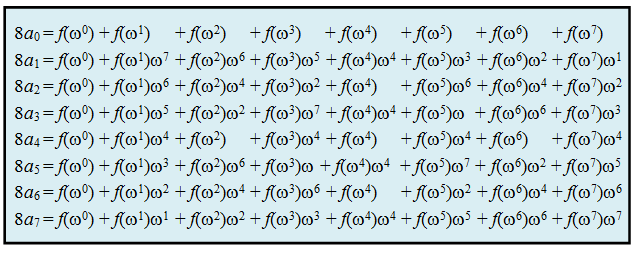
\includegraphics [scale=0.6]{bab2/img/inverse-fft}
	\caption {Inverse Transformasi Fourier Cepat}
	\label {fig:inverse-fft}
\end{figure}
Perhatikan bahwa \textit{Inverse Fast Fourier Transform} hampir sama dengan proses FFT, perbedaannya pada urutan serta $ \omega_N $.

\subsubsection{Number Theoretic Transform} \label{ssec:ntt}
\textit{Number Theoretic Transform} atau NTT didapatkan dengan megeneralisasikan DFT pada $ \mathbb{Z}/p\mathbb{Z} $. NTT biasanya digunakan dalam mengalikan 2 polinomial dalam modulo prima tertentu. Kelebihan NTT adalah tidak ada \textit{precision error} yang sering terjadi pada FFT, karena kalkulasinya menggunakan bilangan integer. Kelemahan utama dari NTT adalah hanya dapat di implementasikan dengan modulo prima yang memenuhi $ p = k \cdot n + 1 $, dimana $ k $ dan $ n $ adalah konstanta tertentu. Sehingga mengimplementasikan NTT dengan bilangan prima acak memerlukan CRT \textit{(Chinese Remainder Theorem)}.

\begin{theo}[Fermat's Little Theorem]
	\label{theo:fermat_little_theorem}
	Jika $ P $ adalah sebuah bilangan prima, maka untuk sembarang integer $ a $, $ a^p - a $ adalah kelipatan dari $ P $.
	\begin{equation}
		\begin{aligned}
			a^{P} \equiv a \Mod{P} \\
			a^{P-1} \equiv 1 \Mod{P} \\
		\end{aligned}
		\label{eq:fermat_theorem}
	\end{equation}
\end{theo}

Pertama, $ \omega_N $ harus berada dalam $ \mathbb{Z}/p\mathbb{Z} $, sedemikian hingga memenuhi persamaan \eqref{eq:root_of_unity_in_z_pz}.
\begin{equation}
	\begin{aligned}
		\omega_N^N = 1 \Mod{P} \\
		P = k \cdot n + 1 \\
	\end{aligned}
	\label{eq:root_of_unity_in_z_pz}
\end{equation}
Menggunakan teorema \ref{theo:fermat_little_theorem}, maka terdapat \textit{primitive root} $ g $, dengan $ x $ dari $ 1 \text{ sampai } P-1 $ maka hasil dari $ g^x \Mod{P} $ berada didalam rentang $ [1,P-1] $ dengan urutan tertentu. Menurut persamaan \eqref{eq:root_of_unity_in_z_pz}, maka didapatkan $ P-1 = k \cdot n $\cite{ntt}. Sehingga 
$$ \omega_n = g^{k} \Mod{P} $$
dan dapat dibuktikan bahwa
$$ \omega_n^n = g^{k \cdot n} = g^{P-1} \equiv 1 \mod{P} $$
$$ \omega_n^m \not\equiv 1 , m < n $$

Oleh karena itu $ \omega_n $ merupakan n\textit{-th primitive root of unity}, yang diperlukan DFT dengan panjang $ n $. Tahap dalam NTT sama seperti FFT pada umunya, perbedaanya hanya pada nilai $ \omega_n $. Nilai dari $ g $ atau generator dapat dilakukan dengan memfaktorkan nilai $ P - 1 $ untuk mendapatkan faktor prima yang unik yang disebut $ upf $. Setelah mendapatkan $ upf $, $ g $ adalah generator apabila memenuhi persamaan \eqref{eq:criteria_of_generator}.
\begin{equation}
	g = \{ a^{\frac{N-1}{p}} \not\equiv 1 \mod{P} | a \in (1,N) , \text{for each } p \text{ in } upf \}
	\label{eq:criteria_of_generator}
\end{equation} 

Perhitungan NTT memerlukan banyak sekali perkalian modular dengan modulo tetap, oleh karena itu NTT dapat diimplementasikan dengan perkalian modular \textit{Montgomery}, untuk mempercepat perkalian modular dalam NTT.

\subsubsection{Perkalian Polinomial menggunakan Number Theoretic Transform}
\label{ssec:langkah_perkalian_ntt}
Operasi perkalian polinomial dapat dioptimasi menggunakan \textit{Number Theoretic Transform} yang telah dibahas pada subbab \ref{ssec:ntt}. Langkah langkah untuk mengalikan polinomial $f(x)$ dan $g(x)$ (konvolusi) dalam modulo $ P $ adalah sebagai berikut :
\begin{enumerate}
	\item \textbf{Praproses} Melakukan penambahan nilai 0 pada polinomial $ f(x) $ atau $ g(x) $ apabila polinomial tersebut tidak memiliki derajat dari hasil pangkat dua pangkat i ($ 2,4,8,16, \cdots $) .
	\item \textbf{Evaluasi NTT} Melakukan evaluasi NTT dari polinomial $ f(x) $ dengan \textit{roots of unity}.
	\item \textbf{Evaluasi NTT} Melakukan evaluasi NTT dari polinomial $ g(x) $ dengan \textit{roots of unity}.
	\item \textbf{Perkalian Titik} Melakukan perkalian titik sehingga $ h(x) = f(x)g(x) $.
	\item \textbf{Interpolasi NTT / Inversi NTT} Melakukan interpolasi titik menggunakan inversi NTT dari $ h(x) $ untuk mendapatkan polinomial dalam representasi koefisien kembali.
\end{enumerate}

\subsection{Pembagian Polinomial}
Didefinisikan 2 buah polinomial $f(x)$ dan $g(x)$ sebagai berikut.
$$ f(x) = a_n x^n + a_{n-1}^{n-1} + \cdots + a_2x^2 + a_1x + a_0 $$
$$ g(x) = b_m x^m + b_{m-1}^{m-1} + \cdots + b_2x^2 + b_1x + b_0 $$
Pembagian ini akan menghasilkan dua polinomial baru $ q(x) $ sebagai hasil bagi dan $ r(x) $ sebagai sisa hasil bagi. Sisa hasil bagi polinomial memiliki beberapa sifat khusus seperti dalam teorema \ref{theo:teorema_sisa_poli}.
Pada umumnya pembagian polinomial dapat dilakukan dengan pembagian secara klasik maupun dengan metode \textit{Horner}, akan tetapi kedua cara tersebut memiliki kompleksitas yang tinggi, oleh karena itu diperlukan algoritma lain dengan kompleksitas lebih rendah. Iterasi Newton dan \textit{Middle Product Optimization} merupakan dua algoritma yang digunakan dalam pembagian polinomial.

\subsubsection{Iterasi Newton}
\indent Misalkan terdapat 2 buah polinomial $f(x)$ dan $g(x)$ dalam $ \mathbb{Z}/p\mathbb{Z} $ sebagai berikut.
$$ f(x) = a_{2n-2} x^{2n-2} + \cdots + a_2x^2 + a_1x + a_0 $$
$$ g(x) = b_{n-1} x^{n-1} + \cdots + b_2x^2 + b_1x + b_0 $$
Ketika membagi $ f $ dengan $ g $ didapatkan hubungan sebagai berikut $ f = qg + r $.
Misalkan 
$$ f^*(x) = x^{2n-2}f(1/x) = a_0 x^{2n-2} + \cdots + a_{2n-2} $$
$$ g^*(x) = x^{n-1}g(1/x) = b_0 x^{n-1} + \cdots + b_{n-1} $$
sehingga $ f^* $ dan $ g^* $ merupakan polinomial dengan urutan terbalik dari $ f $ dan $ g $, kemudian
\begin{equation}
	f(x) = q(x)g(x) + r(x) \iff f^*(x) = q*(x) g*(x) + x^{n-1+\lambda} r*(x)
	\label{eq:persamaan_reversal}
\end{equation}
dengan $ \lambda \geq 1 $. Maka didapatkan nilai $ q* $ sehingga dapat menghitung nilai dari sisanya atau $ r* $ dengan $ f-qg $.

Iterasi newton merupakan algortima iteratif untuk mengaproksimasi solusi dari fungsi non-linear $ f(x) = 0 $. Iterasi dimulai dengan dugaan awal nilai tertentu, yang konvergen dengan fungsi $ f(x) $. 
Didefinisikan \textit{power series} $ \bar{p}(x) $ adalah aproksimasi polinomial derajat $ n $ dari $ p(x) $ sehingga $ \bar{p}(x) = P(x) + O(x^n) = p(x) \mod{x^n} $. 
Apabila $ y(x) = g(x)^{-1} $, mencari $ y(x) $ ekivalen dengan mencari solusi dari persamaan $$ a(x) - \frac{1}{y(x)} = 0. $$

Didefinisikan $ f(y) = a(x) - \frac{1}{y} $, serta $ f(y_k) + f^{'}(y_k)(Y_{k+1} - y_k) = 0 $, maka dihasilkan persamaan \eqref{eq:persamaan_iterasi_newton}.
\begin{equation}
	\begin{aligned}
		y_{k+1} &= y_k - \frac{f(y_k)}{f^{'}(y_k)} \\
				&= y_k - \frac{a(x) - \frac{1}{y_k}}{\frac{1}{y_k^2}} \\
				&= y_k + y_k(1 - y_k \cdot a(x)).
	\end{aligned}
	\label{eq:persamaan_iterasi_newton}
\end{equation}
Untuk mencari nilai dari $ q* $, diawali dengan mencari nilai dari $ \frac{1}{g(x)} $, dengan menggunakan iterasi newton memerlukan nilai awal $ y_0 = \frac{1}{g_{n-1}} $ atau inverse dari konstant, kemudian dilanjutkan untuk $ k $ dari $ 1 $ hingga $ \log_2 n $ menggunakan persamaan \eqref{eq:iterasi_newton}.
\begin{equation}
	y_k \equiv 2y_{k-1} - y_{k-1}^2 b^* \mod{x^{2^{k}}}
	\label{eq:iterasi_newton}
\end{equation}
Sehingga untuk menghitung nilai dari $ q* $ dapat menggunakan persamaan \eqref{eq:q_star}.
\begin{equation}
	q^* = f^* \cdot \frac{1}{g^*} \mod{x^n}
	\label{eq:q_star}
\end{equation}
Sehingga pada setiap step memerlukan 3 kali perkalian polinomial dan 1 kali perkalian polinomial untuk mendapatkan nilai dari $ q* $. Untuk mendapatkan nilai dari $ r $ menggunakan persamaan $ r = f-gq $ memerlukan 1 kali perkalian polinomial kembali. Sehingga iterasi newton memerlukan banyak sekali perkalian polinomial. Operasi ini dapat dioptimasi apabila digunakan perkalian polinomial berbasis FTT/NTT.

\subsubsection{Middle Product Optimization}
\indent Misal $ n = 2^k $, kemudian diketahui bahwa
$$ y_k \equiv 2y_{k-1} - y_{k-1}^2 b^* \mod{x^{2^{k}}} = y_{k-1} + y_{k-1}(1 - b^* y_{k-1}) \mod{x^{2^k}}. $$
Dalam keadaan normal, perkalian polinomial dengan derajat $ 2n - 1 $ dan $ n - 1 $ memerlukan perkalian polinomial berbasis NTT dengan \textit{array} yang bisa menampung setidaknya $ 3n $ elemen. Tetapi perkalian polinomial berbasis NTT memerlukan input dengan ukuran pangkat dua, sehingga memerlukan \textit{array} dengan ukuran $ 4n $. Diketahui bahwa $ 1-y_kb^* \equiv 0 \mod{x^{2^k}} $, sehingga perkalian $ y_kb^* $ akan menghasilkan polinomial seperti dalam persamaan \eqref{eq:persamaan_asal_mula_m(x)}, dengan $ h(x) = 1 + 0 \cdot x + \cdots + 0 \cdot x^{n-1}. $
\begin{equation}
	\begin{aligned}
y_k \cdot b^* &= h(x) + m_0 \cdot x^n + m_1 \cdot x^{n+1} + \cdots + m_n-1 \cdot x^{2n-1} + O(x^{2n}) \\
			  &= h(x) + x^n ( m_0 + m_1 \cdot x + \cdots + m_n-1 \cdot x^{n-1}) + O(x^{2n}) \\
			  &= h(x) + x^n m(x) + (c_0 + c_1 \cdot x + \cdots + c_{n-1} \cdot x^{n-1} ) \\
	\end{aligned}
	\label{eq:persamaan_asal_mula_m(x)}
\end{equation}
$$ \text{dimana } m(x) = m_0 + m_1 \cdot x + \cdots + m_n-1 \cdot x^{n-1}. $$

Sehingga bisa didefinisikan \textit{field} $ F $ dan polinomial $ a(x) $ yang merupakan \textit{power series} dalam $ F[[x]] $ dengan $ a_0 \neq 0 $. Untuk sembarang integer $ n \geq 2 $, misal $ b = a(x) \mod{x^n} $, dan $ y = a(x)^{-1} \mod{x^m} $ dengan $ m = \lceil \frac{n}{2} \rceil $. Jika 
$$ y \cdot b = \sum_{i=0}^{n+m-2}g_ix^i, $$ maka polinomial $$ \sum_{i=0}^{n-m+1} g_{m+i} x^i $$ disebut dengan \textit{Middle Product}.
Menggunakan definisi diatas, dapat didefinisikan teorema \ref{theo:middle_product}\cite{middle_product_op}.

\begin{theo}[Middle Product]
	\label{theo:middle_product}
	Misal $ F,a(x),n,b,m \text{ dan } y $ sama seperti definisi diatas, serta $ N $ adalah bilangan pangkat 2 sehingga $ N/2 < n \leq N $ dan $ \omega $ merupakan \textit{N-th primitive root of unity}. Jika
		$$ FFT(b,N,\omega) = (B_0, B_1, \cdots, B_{N-1}), $$
		$$ FFT(y,N,\omega) = (Y_0, Y_1, \cdots, Y_{N-1}), $$
		$$ D_i = B_i \cdot Y_i \text{ untuk i } = 0, \cdots N-1 \text{ dan } $$
		$$ (d_0, d_1, \cdots , d_{N-1}) = N^{-1} FFT(\sum_{i=0}^{N-1} D_iX^i, N, \omega^-1), \text{ sehingga } $$
		$$ \text{MP } = \sum_{i=0}^{n-m+1} d_{m+i}x^i. $$
		\label{eq:middle_product}
\end{theo}

Menggunakan metode optimasi ini dapat mengurangi jumlah pemanggilan FFT/NTT dengan mengurangi ukuran \textit{array} pada perkalian FFT/NTT dari $ 2n $ menjadi $ n $. Proses perkalian FFT/NTT pada teorema \ref{theo:middle_product} merupakan FFT/NTT dengan konvolusi \textit{cyclic}. Pseudocode \ref{psdo:middle_product} menggambarkan proses dari Middle Product Optimization.

\begin{algorithm}
	\caption{MiddleProduct}
	\label{psdo:middle_product}
	\begin{algorithmic}[1]
		\Require $ a $
		\Ensure $ a(x)^{-1} $
		\State $ y \leftarrow \frac{1}{a_0} $
		\State $ N \leftarrow 1 $
		\While{$N < n$}
			\State $ N \leftarrow 2 * N $
			\State $ b \leftarrow a(x) \text{ mod } x^N $
			\State $ y \leftarrow y(1- y.b) \text{ mod } x^N $
		\EndWhile
		\State \Return $ y \text{ mod } x^n $
	\end{algorithmic}
\end{algorithm}


\subsubsection{Pembagian Polinomial menggunakan Iterasi Newton dan Middle Product Optimization}
Pada subbab ini akan dibahas mengenai pembagian polinomial menggunakan Iterasi Newton dan Middle Product Optimization. Didefinisikan operasi $ rev_k(a) = x^ka(1/x) $. Ketika $ k = n $ maka akan didapatkan polinomial a dengan koefisien yang dibalik. Apabila persamaan \eqref{eq:persamaan_reversal} ditulis kembali dengan melibatkan operasi $ rev_k(a) $, maka didapatkan persamaan \eqref{eq:persamaan_reversal_baru}.
\begin{equation}
	rev_n(f) = rev_{n-m}(q).rev_m(g)+x^{n-m+1}rev_{m-1}(r)
	\label{eq:persamaan_reversal_baru}
\end{equation}
Sehingga didapatkan sebagai berikut
\begin{equation}
	\begin{aligned}
		q &= rev_{n-m}(rev_{n}(f) \cdot rev_{m}(g)^{-1} \text{ mod } x^{n - m + 1}) \\
		r &= f - q.g
	\end{aligned}
\end{equation}

Selain menggunakan rumus diatas, nilai dari $ q $ dapat dihitung dengan memanfaatkan sifat dari Middle Product disertai Iterasi Newton. Pseudocode \ref{psdo:pembagian_poli_mp} merupakan pseudocode pembagian polinomial berdasarkan \cite{middle_product_hal} dan \cite{middle_product_op} yang melibatkan Middle Product Optimization dan Iterasi Newton. 

\begin{algorithm}
	\caption{Pembagian Polinomial dengan MP}
	\label{psdo:pembagian_poli_mp}
	\begin{algorithmic}[1]
		\Require $a = [a_0, a_1, \cdots, a_{n-1}], b = [b_0, b_1, \cdots, b_{n-1}]$
		\If{$ n = 1 $} 
		\State \Return $ \left [b_0/a_0\right ] $ 
		\EndIf
		\State $ p \leftarrow \left \lfloor \frac{n}{2} \right \rfloor $
		\State $ inv \leftarrow b_{[0 \cdots n - p - 1]}^{-1} $
		\State $ q1 \leftarrow inv \times a_{[0 \cdots n - p - 1]} $
		\State $ lo \leftarrow \Call{\fakesc{MiddleProduct}}{q1, b} $
		\State $ q2 \leftarrow \left[ inv_0, \cdots inv_{p-1} \right] \times \left[ b_{n-p} - lo_{0}, \cdots,  b_{n-1} - lo_{p-1} \right] $
		\State \Return $ [q1_0, \cdots, q1_{n-p-1}, q2_0, \cdots, q2_{p-1}] $.
	\end{algorithmic}
\end{algorithm}

\section{Strategi Optimasi}
Pada subbab ini akan dipaparkan metode optimasi yang digunakan dalam tugas akhir ini. Secara singkat terdapat 2 strategi optimasi yang digunakan dalam tugas akhir ini yaitu :
\begin{enumerate}
	\item Optimasi Operasi Perkalian Modulo
	\item Optimasi Operasi Pemangkatan Modulo
	\item Optimasi Perhitungan Prima yang digunakan dalam NTT
\end{enumerate}

\subsection{Optimasi Operasi Perkalian Modulo}
Optimasi Perkalian Modulo dapat dilakukan dengan menerapkan Perkalian Modular \textit{Montgomery}. Perkalian Modular \textit{Montgomery} atau reduksi \textit{montgomery} adalah metode efisien untuk menghitung $ u = a \cdot b \Mod{n} $ dengan $ a, b, $ dan $ n $ adalah  bilangan $k$-bit, yang dikenalkan oleh Peter L. Montgomery pada tahun 1985 \cite{montgomery}. 

Algoritma ini cocok digunakan dalam implementasi pada software dan hardware komputer karena kemampuannya dalam melakukan operasi modulo pangkat 2 dengan cepat. Reduksi untuk menghasilkan $ u $ tidak dilakukan dengan cara pembagian dengan $ n $ seperti pada perkalian modulo pada umumnya, tetapi dengan $ 2^r $ dalam representasi \textit{Montgomery World}.

Asumsikan modulus $ n $ adalah bilangan $k$-bit sedemikian hingga $ 2^{k-1} \leq n < 2^{k} $ dan $ r = 2^{k}$. Perkalian modular \textit{montgomery} memerlukan nilai $ r $ dan $ n $ yang relatif prima sedemikian hingga $ gcd(r, n) = gcd(2^k, n) = 1 $. Persamaan diatas dapat dipenuhi apabila $ n $ adalah bilangan ganjil.

Diberikan bilangan bulat $ a < n $ dan $ b < n $, yang dalam representasi \textit{Montgomery World} dengan $ r $ dilambangkan dalam persamaan \eqref{eq:mont_world}
\begin{equation}
	\begin{aligned}
		\bar{a} = a \cdot r \Mod{n} \\
		\bar{b} = b \cdot r \Mod{n} \\
	\end{aligned}
	\label{eq:mont_world}
\end{equation}
Perkalian modular \textit{montgomery} didefinisikan dalam persamaan \eqref{eq:mont_mul}
\begin{equation}
	x = \bar{a} \cdot \bar{b} \cdot r^{-1} \Mod{n}
	\label{eq:mont_mul}
\end{equation}
dengan $ r^{-1} $ adalah modulo inverse dari $ r $ dalam modulo $ n $. Langkah selanjutnya adalah reduksi, dalam reduksi \textit{montgomery} memperlukan nilai dari $ n' $ yang bisa didapatkan melalui identitas \eqref{eq:mont_identitas}
\begin{equation}
	r \cdot r^{-1} - n \cdot n' = 1
	\label{eq:mont_identitas}
\end{equation}
sehingga nilai $ n' $ dilambangkan persamaan \eqref{eq:mont_n_aksen}
\begin{equation}
	n' = \frac{r(r^{-1}\mod{n}) -1}{n}
	\label{eq:mont_n_aksen}
\end{equation}

Perkalian modular \textit{montgomery} lebih cocok digunakan dalam \textit{chain multiplication} dengan modulo tetap, sehingga algoritma ini dapat digunakan dalam pemangkatan modular cepat.Algoritma perkalian modular \textit{montgomery} dapat dirangkum dalam pseudocode \ref{psdo:montgomery}. 

\begin{algorithm}
	\caption{Perkalian Modular Montgomery}
	\label{psdo:montgomery}
	\begin{algorithmic}[1]
		\Require $a,\ b,\ n$
		\Ensure $c = ab\mod{n}$
		\State $r = 2^n $, $ r \in \mathbb{N}, r > n, gcd(r,n) = 1 $
		\State $n' = \frac{r(r^{-1}\mod{n}) -1}{n} $
		\State $\bar{a} = a \cdot r \Mod{n} $
		\State $\bar{b} = b \cdot r \Mod{n} $
		\State $x = \bar{a}\bar{b} $
		\State $s = (x \cdot n'\ \mod{r}) $
		\State $t = x + sn $
		\State $u = \frac{t}{r} $
		\If{$u < n$}
			$\ \bar{c} = u $
		\Else
			$\ \bar{c} = u - n $
		\EndIf \\
		\Return $ c = \bar{c}r^{-1}\mod{n} $.
	\end{algorithmic}
\end{algorithm}

Selain perkalian, \textit{montgomery} bisa diterapkan untuk operasi seperti pertambahan dan pengurangan, karena sifat distribusi yang dimiliki modulo.
$$ ar + br = (a+b)r $$
$$ ar - br = (a-b)r $$
Sementara untuk operasi pembagian, hampir sama dengan pembagian modular biasa, dengan mengalikan dalam \textit{Montgomery World} dengan inversenya.
$$ \frac{a}{b}r = ar \cdot b^{-1}r $$

\subsection{Optimasi Operasi Pemangkatan Modulo}
Operasi perpangkatan diperlukan dalam perhitungan modulo inverse dari $ b $ dalam modulo $ n $. Dengan metode naif, operasi pemangkatan memerlukan kompleksitas $ \mathcal{O}{(n)} $.
$$ a^n = a \cdot a \cdots a\ (n\ kali) $$

Namun, hasil yang sama bisa diperoleh dengan kompleksitas lebih rendah, jika menggunakan metode \textit{fast modular exponentiation}, yaitu mengubah bilangan pemangkat yaitu $ n $ menjadi basis biner terlebih dahulu, lalu dilakukan perkalian bertahap, untuk contoh dalam menghitung nilai dari $ x^{11} $
$$ x^{11} = x^{1+2+8} = (x)(x^{2})(x^{8}) $$
atau dalam kongruensi 
$$ x^{11}\ \mod{n} \equiv [(x\mod{n})(x^{2}\mod{n})(x^{8}\mod{n})]\mod{n} $$

Secara umum, apabila menghitung nilai dari $ a^b\mod{n} $, dengan $ a $ dan $ b $ adalah bilangan bulat, maka kita bisa mengubah $ b $ dalam basis biner $b_{k} b_{k-1} b_{k-2} \cdots b_{0}$, seperti persamaan \eqref{eq:basis_biner_b}.

\begin{equation}
	b = \sum_{b_i \neq 0} 2^i
	\label{eq:basis_biner_b}
\end{equation}

Kemudian, dengan mensubstitusikan $ b $ dari persamaan \eqref{eq:basis_biner_b}, didapatkan persamaan \eqref{eq:modular_expo}.

$$ a^b = a^{\sum_{b_i \neq 0} 2^i} = \prod_{b_i \neq 0} a^{2^{i}} $$
\begin{equation}
	a^b\mod{n} = \left [ \prod_{b_i \neq 0} a^{2^{i}} \mod{n} \right ] \mod{n}
	\label{eq:modular_expo}
\end{equation}

Dalam menghitung nilai dari $ a^{2^{i}} $, dapat dilakukan secara iteratif, sehingga persamaan \eqref{eq:modular_expo} dapat ditulis kembali menjadi persamaan \eqref{eq:modular_expo_f_y}.

\begin{equation}
	\begin{aligned}
	a^b\mod{n} = \left [ \prod_{k = 1} f_y(k)\right ] \mod{n} \\
	f_y(k)=
		\begin{cases}
			1,  					& \text{if } b_k=0 \\
			a^{2^{k}}  \mod{n} ,   & \text{if } b_k=1
		\end{cases} \\
	\end{aligned}
	\label{eq:modular_expo_f_y}
\end{equation}

Dengan persamaan \eqref{eq:modular_expo_f_y} dapat dibuktikan perhitungan $ a^b \mod{n} $ membutuhkan $ log_2\ b $ perkalian, sehingga \textit{fast modular exponentiation} atau perpangkatan modular \textit{repeated squaring} memiliki kompleksitas $ \mathcal{O}{(log_2\ n)} $. Berikut merupakan pseudocode untuk \textit{fast modular exponentiation}.
\begin{algorithm}
	\caption{Fast Modular Exponentiation}
	\label{psdo:fast_modex}
	\begin{algorithmic}[1]
		\Require $a,\ b,\ n$
		\Ensure $y = a^b\mod{n}$
		\State $y \leftarrow 1$
		\While{ $ b > 0 $}
			\If {$ b $\ is\ odd}
				\State $ y = y \cdot a $
			\EndIf
			\State $ b = b / 2 $
			\State $ a = a \cdot a $
		\EndWhile \\
		\Return $ y $
	\end{algorithmic}
\end{algorithm}

\subsubsection{Optimasi Perhitungan Prima yang digunakan dalam NTT}

Dikarenakan permasalahan \soal, terdapat modulo yang berbeda untuk kasus uji yang berbeda, sehingga untuk setiap kasus uji diharuskan untuk mencari generator baru untuk NTT, yang mana akan memiliki kompleksitas lebih. Oleh karena itu penulis menggunakan algoritma \textit{Chineese Remainder Theorem} atau CRT untuk mengeneralisasikan hasil berdasarkan beberapa kongruensi prima tetap. Bilangan prima yang digunakan harus lebih besar dari batas prima yang menjadi masukan pada permasalahan.

\textit{Chinese Remainder Theorem} merupakan teorema dalam teori bilangan yang dikembangkan oleh Sunzi pada tahun 201 - 300.
\begin{theo}[Chinese Remainder Theorem]
	\label{theo:chinese_remainder_theorem}
	Diberikan pasangan bilangan yang saling \textit{coprime} $n_1, n_2, \cdots, n_k$ dan sembarang bilangan $ a_1, a_2, \cdots, a_k $, dengan sistem konguensi 
	\begin{equation}
		\begin{aligned}
		x &\equiv a_1 \Mod{n_1}\\
		x &\equiv a_2 \Mod{n_2}\\
		& \vdots\\
		x &\equiv a_k \Mod{n_k}\\
		\end{aligned}
	\end{equation}
	mempunyai solusi, dan solusi adalah unik dalam modulo $ N = n_1n_2\cdots n_k$.
\end{theo}
Bedasarkan teorema \ref{theo:chinese_remainder_theorem}, bisa disusun langkah dalam menyelesaikan sistem kongruensi\cite{brilliant_crt}. 
\begin{enumerate}
	\item Hitung $ N = n_1 \times n_2 \times \cdots \times n_k$.
	\item Untuk setiap $ i = 1,2,\cdots,k $ hitung $$ y_i = \frac{N}{n_i} $$.
	\item Untuk setiap $ i = 1,2,\cdots,k $ hitung $ z_i = y_i^{-1} \mod{n_i} $.
	\item Solusi sistem kongruensi adalah integer $ x = \sum_{i=1}^{k} a_i y_i z_i $, dengan $ x \mod{N} $ adalah solusi unik dari modulo $ N $
\end{enumerate}
Terdapat \textit{case} khusus dalam menyelesaikan sistem kongruensi dengan $ k = 2 $.
$$ x \equiv a_1 \Mod{n_1} $$
$$ x \equiv a_2 \Mod{n_2} $$
dengan $ n_1 \text{ dan } n_2 $ saling \textit{coprime}.
Menggunakan \textit{Bézout's identity} yang mengatakan bahwa terdapat dua bilangan $ m_1 \text{ dan } m_2 $ sehingga 
\begin{equation}
	m_1 n_1 + m_2 n_2 = 1.
	\label{eq:bezeout_identity}
\end{equation}
Sehingga solusi sistem kongruensi diberikan $ x = a_1 m_2 n_2 + a_2 m_1 n_1 $, dapat diubah menjadi persamaan \eqref{eq:crt_2_modulo}.
\begin{equation}
	\begin{aligned}
		x &= a_1 m_2 n_2 +a_2 m_1n_1 \\
		  &= a_1 (1-m_1 n_1) + a_2 m_1 n_1 \\
		  &= a_1 +( a_2-a_1) m_1 n_1.
	\end{aligned}
	\label{eq:crt_2_modulo}
\end{equation}

Apabila persamaan \eqref{eq:crt_2_modulo}, dihitung dalam modulo $ p $ yang menjadi input, maka persamaan $ x $ akan menjadi penyelesaian sistem kongruensi dalam modulo $ p $, sesuai dengan permasalahan. Untuk permasalahan ini, penulis menggunakan 2 bilangan prima yang tercantum pada tabel \ref{tab:two_primes} yang digunakan sebagai dasar modulo perhitungan NTT. Bilangan prima tersebut dipilih karena memenuhi syarat modulo bilangan prima pada NTT dan memiliki nilai lebih dari $ 10^{11} $.

\begin{table}[]
	\Centering
	\begin{tabular}{|c|c|}
	\hline
	Prima              & Generator \\ \hline
	709143768229478401 & 31        \\ \hline
	711416664922521601 & 19        \\ \hline
	\end{tabular}
	\caption{Modulo bilangan prima yang digunakan dalam perhitungan NTT}
	\label{tab:two_primes}
\end{table}
